
%\documentclass[11pts,a4paper,amsmath,amssymb,floatfix]{article}%{report}%{book}
\documentclass[12pts,a4paper,amsmath,amssymb,floatfix]{article}%{report}%{book}
\usepackage{graphicx,wrapfig,pdfpages}% Include figure files
%\usepackage{dcolumn,enumerate}% Align table columns on decimal point
\usepackage{enumerate,enumitem}% Align table columns on decimal point
\usepackage{bm,dpfloat}% bold math
\usepackage[pdftex,bookmarks,colorlinks=true,urlcolor=rltblue,citecolor=blue]{hyperref}
\usepackage{amsfonts,amsmath,amssymb,stmaryrd,indentfirst}
\usepackage{times,psfrag}
\usepackage{natbib}
\usepackage{color}
\usepackage{units}
\usepackage{rotating}
\usepackage{multirow}


\usepackage{pifont}
\usepackage{subfigure}
\usepackage{subeqnarray}
\usepackage{ifthen}

\usepackage{supertabular}
\usepackage{moreverb}
\usepackage{listings}
\usepackage{palatino}
%\usepackage{doi}
\usepackage{longtable}
\usepackage{float}
\usepackage{perpage}
\MakeSorted{figure}
%\usepackage{pdflscape}


%\usepackage{booktabs}
%\newcommand{\ra}[1]{\renewcommand{\arraystretch}{#1}}


\definecolor{rltblue}{rgb}{0,0,0.75}


%\usepackage{natbib}
\usepackage{fancyhdr} %%%%
\pagestyle{fancy}%%%%
% with this we ensure that the chapter and section
% headings are in lowercase
%%%%\renewcommand{\chaptermark}[1]{\markboth{#1}{}}
\renewcommand{\sectionmark}[1]{\markright{\thesection\ #1}}
\fancyhf{} %delete the current section for header and footer
\fancyhead[LE,RO]{\bfseries\thepage}
\fancyhead[LO]{\bfseries\rightmark}
\fancyhead[RE]{\bfseries\leftmark}
\renewcommand{\headrulewidth}{0.5pt}
% make space for the rule
\fancypagestyle{plain}{%
\fancyhead{} %get rid of the headers on plain pages
\renewcommand{\headrulewidth}{0pt} % and the line
}

\def\newblock{\hskip .11em plus .33em minus .07em}
\usepackage{color}

%\usepackage{makeidx}
%\makeindex

\setlength\textwidth      {16.cm}
\setlength\textheight     {22.6cm}
\setlength\oddsidemargin  {-0.3cm}
\setlength\evensidemargin {0.3cm}

\setlength\headheight{14.49998pt} 
\setlength\topmargin{0.0cm}
\setlength\headsep{1.cm}
\setlength\footskip{1.cm}
\setlength\parskip{0pt}
\setlength\parindent{0pt}


%%%
%%% Headers and Footers
\lhead[] {\text{\small{EG501J -- Geothermal Energy}}} 
\rhead[] {{\text{\small{Tutorial 01}}}}
%\chead[] {\text{\small{Session 2012/13}}} 
\lfoot[]{Dr Jeff Gomes}
%\cfoot[\thepage]{\thepage}
\rfoot[\text{\small{\thepage}}]{\thepage}
\renewcommand{\headrulewidth}{0.8pt}


%%%
%%% space between lines
%%%
\renewcommand{\baselinestretch}{1.5}

\newenvironment{VarDescription}[1]%
  {\begin{list}{}{\renewcommand{\makelabel}[1]{\textbf{##1:}\hfil}%
    \settowidth{\labelwidth}{\textbf{#1:}}%
    \setlength{\leftmargin}{\labelwidth}\addtolength{\leftmargin}{\labelsep}}}%
  {\end{list}}

%%%%%%%%%%%%%%%%%%%%%%%%%%%%%%%%%%%%%%%%%%%
%%%%%%                              %%%%%%%
%%%%%%      NOTATION SECTION        %%%%%%%
%%%%%%                              %%%%%%%
%%%%%%%%%%%%%%%%%%%%%%%%%%%%%%%%%%%%%%%%%%%

% Text abbreviations.
\newcommand{\ie}{{\em{i.e., }}}
\newcommand{\eg}{{\em{e.g., }}}
\newcommand{\cf}{{\em{cf., }}}
\newcommand{\wrt}{with respect to}
\newcommand{\lhs}{left hand side}
\newcommand{\rhs}{right hand side}
% Commands definining mathematical notation.

% This is for quantities which are physically vectors.
\renewcommand{\vec}[1]{{\mbox{\boldmath$#1$}}}
% Physical rank 2 tensors
\newcommand{\tensor}[1]{\overline{\overline{#1}}}
% This is for vectors formed of the value of a quantity at each node.
\newcommand{\dvec}[1]{\underline{#1}}
% This is for matrices in the discrete system.
\newcommand{\mat}[1]{\mathrm{#1}}


\DeclareMathOperator{\sgn}{sgn}
\newtheorem{thm}{Theorem}[section]
\newtheorem{lemma}[thm]{Lemma}

%\newcommand\qed{\hfill\mbox{$\Box$}}
\newcommand{\re}{{\mathrm{I}\hspace{-0.2em}\mathrm{R}}}
\newcommand{\inner}[2]{\langle#1,#2\rangle}
\renewcommand\leq{\leqslant}
\renewcommand\geq{\geqslant}
\renewcommand\le{\leqslant}
\renewcommand\ge{\geqslant}
\renewcommand\epsilon{\varepsilon}
\newcommand\eps{\varepsilon}
\renewcommand\phi{\varphi}
\newcommand{\bmF}{\vec{F}}
\newcommand{\bmphi}{\vec{\phi}}
\newcommand{\bmn}{\vec{n}}
\newcommand{\bmns}{{\textrm{\scriptsize{\boldmath $n$}}}}
\newcommand{\bmi}{\vec{i}}
\newcommand{\bmj}{\vec{j}}
\newcommand{\bmk}{\vec{k}}
\newcommand{\bmx}{\vec{x}}
\newcommand{\bmu}{\vec{u}}
\newcommand{\bmv}{\vec{v}}
\newcommand{\bmr}{\vec{r}}
\newcommand{\bma}{\vec{a}}
\newcommand{\bmg}{\vec{g}}
\newcommand{\bmU}{\vec{U}}
\newcommand{\bmI}{\vec{I}}
\newcommand{\bmq}{\vec{q}}
\newcommand{\bmT}{\vec{T}}
\newcommand{\bmM}{\vec{M}}
\newcommand{\bmtau}{\vec{\tau}}
\newcommand{\bmOmega}{\vec{\Omega}}
\newcommand{\pp}{\partial}
\newcommand{\kaptens}{\tensor{\kappa}}
\newcommand{\tautens}{\tensor{\tau}}
\newcommand{\sigtens}{\tensor{\sigma}}
\newcommand{\etens}{\tensor{\dot\epsilon}}
\newcommand{\ktens}{\tensor{k}}
\newcommand{\half}{{\textstyle \frac{1}{2}}}
\newcommand{\tote}{E}
\newcommand{\inte}{e}
\newcommand{\strt}{\dot\epsilon}
\newcommand{\modu}{|\bmu|}
% Derivatives
\renewcommand{\d}{\mathrm{d}}
\newcommand{\D}{\mathrm{D}}
\newcommand{\ddx}[2][x]{\frac{\d#2}{\d#1}}
\newcommand{\ddxx}[2][x]{\frac{\d^2#2}{\d#1^2}}
\newcommand{\ddt}[2][t]{\frac{\d#2}{\d#1}}
\newcommand{\ddtt}[2][t]{\frac{\d^2#2}{\d#1^2}}
\newcommand{\ppx}[2][x]{\frac{\partial#2}{\partial#1}}
\newcommand{\ppxx}[2][x]{\frac{\partial^2#2}{\partial#1^2}}
\newcommand{\ppt}[2][t]{\frac{\partial#2}{\partial#1}}
\newcommand{\pptt}[2][t]{\frac{\partial^2#2}{\partial#1^2}}
\newcommand{\DDx}[2][x]{\frac{\D#2}{\D#1}}
\newcommand{\DDxx}[2][x]{\frac{\D^2#2}{\D#1^2}}
\newcommand{\DDt}[2][t]{\frac{\D#2}{\D#1}}
\newcommand{\DDtt}[2][t]{\frac{\D^2#2}{\D#1^2}}
% Norms
\newcommand{\Ltwo}{\ensuremath{L_2} }
% Basis functions
\newcommand{\Qone}{\ensuremath{Q_1} }
\newcommand{\Qtwo}{\ensuremath{Q_2} }
\newcommand{\Qthree}{\ensuremath{Q_3} }
\newcommand{\QN}{\ensuremath{Q_N} }
\newcommand{\Pzero}{\ensuremath{P_0} }
\newcommand{\Pone}{\ensuremath{P_1} }
\newcommand{\Ptwo}{\ensuremath{P_2} }
\newcommand{\Pthree}{\ensuremath{P_3} }
\newcommand{\PN}{\ensuremath{P_N} }
\newcommand{\Poo}{\ensuremath{P_1P_1} }
\newcommand{\PoDGPt}{\ensuremath{P_{-1}P_2} }

\newcommand{\metric}{\tensor{M}}
\newcommand{\configureflag}[1]{\texttt{#1}}

% Units
\newcommand{\m}[1][]{\unit[#1]{m}}
\newcommand{\km}[1][]{\unit[#1]{km}}
\newcommand{\s}[1][]{\unit[#1]{s}}
\newcommand{\invs}[1][]{\unit[#1]{s}\ensuremath{^{-1}}}
\newcommand{\ms}[1][]{\unit[#1]{m\ensuremath{\,}s\ensuremath{^{-1}}}}
\newcommand{\mss}[1][]{\unit[#1]{m\ensuremath{\,}s\ensuremath{^{-2}}}}
\newcommand{\K}[1][]{\unit[#1]{K}}
\newcommand{\PSU}[1][]{\unit[#1]{PSU}}
\newcommand{\Pa}[1][]{\unit[#1]{Pa}}
\newcommand{\kg}[1][]{\unit[#1]{kg}}
\newcommand{\rads}[1][]{\unit[#1]{rad\ensuremath{\,}s\ensuremath{^{-1}}}}
\newcommand{\kgmm}[1][]{\unit[#1]{kg\ensuremath{\,}m\ensuremath{^{-2}}}}
\newcommand{\kgmmm}[1][]{\unit[#1]{kg\ensuremath{\,}m\ensuremath{^{-3}}}}
\newcommand{\Nmm}[1][]{\unit[#1]{N\ensuremath{\,}m\ensuremath{^{-2}}}}

% Dimensionless numbers
\newcommand{\dimensionless}[1]{\mathrm{#1}}
\renewcommand{\Re}{\dimensionless{Re}}
\newcommand{\Ro}{\dimensionless{Ro}}
\newcommand{\Fr}{\dimensionless{Fr}}
\newcommand{\Bu}{\dimensionless{Bu}}
\newcommand{\Ri}{\dimensionless{Ri}}
\renewcommand{\Pr}{\dimensionless{Pr}}
\newcommand{\Pe}{\dimensionless{Pe}}
\newcommand{\Ek}{\dimensionless{Ek}}
\newcommand{\Gr}{\dimensionless{Gr}}
\newcommand{\Ra}{\dimensionless{Ra}}
\newcommand{\Sh}{\dimensionless{Sh}}
\newcommand{\Sc}{\dimensionless{Sc}}


% Journals
\newcommand{\IJHMT}{{\it International Journal of Heat and Mass Transfer}}
\newcommand{\NED}{{\it Nuclear Engineering and Design}}
\newcommand{\ICHMT}{{\it International Communications in Heat and Mass Transfer}}
\newcommand{\NET}{{\it Nuclear Engineering and Technology}}
\newcommand{\HT}{{\it Heat Transfer}}   
\newcommand{\IJHT}{{\it International Journal for Heat Transfer}}

\newcommand{\frc}{\displaystyle\frac}

\newlist{ExList}{enumerate}{1}
\setlist[ExList,1]{label={\bf Example 1.} {\bf \arabic*}}

\newlist{ProbList}{enumerate}{1}
\setlist[ProbList,1]{label={\bf Problem 1.} {\bf \arabic*}}

%%%%%%%%%%%%%%%%%%%%%%%%%%%%%%%%%%%%%%%%%%%
%%%%%%                              %%%%%%%
%%%%%% END OF THE NOTATION SECTION  %%%%%%%
%%%%%%                              %%%%%%%
%%%%%%%%%%%%%%%%%%%%%%%%%%%%%%%%%%%%%%%%%%%


% Cause numbering of subsubsections. 
%\setcounter{secnumdepth}{8}
%\setcounter{tocdepth}{8}

\setcounter{secnumdepth}{4}%
\setcounter{tocdepth}{4}%


\begin{document}



\begin{enumerate}[label=\bfseries Problem \arabic*:]
%

%%%
%%%
%%%
\item\label{EasyQuestion} {\it Data below indicates how temperature varies with depth in a hypothetical geothermal electricity site. 
\begin{center}
\begin{tabular}{||c | c | c | c| c | c| c ||}
\hline\hline
{\bf Temperature $\left(^{o}C\right)$} & 25 & 40 & 63 & 100 & 155 & 245 \\
{\bf Depth (m)}                        & 0 & 200 & 400 & 600 & 800 & 1000 \\
\hline\hline
\end{tabular}
\end{center}
\begin{enumerate}
\item Plot the diagram depth $\times$ temperature. 
\item The power plant you are designing is operated with groundwater at 225$^{o}$C. Assuming there is no heat loss from the geothermal source to the environment, determine the depth that it is necessary to drill to produce hot stream for the plant facility.
\item Part of the water used to generate electricity is also used in a district heating system with flow and return temperatures of 80$^{o}$C and 60$^{o}$C respectively.  10$\%$ of the energy supplied is lost in distribution.  A total heat demand on a typical winters day from all building connected to the system is 20 MW. The current heating is supplied by a coal fired boiler operating at an efficiency of 80$\%$.  How much coal is consumed each day if the calorific value of the coal is 24 GJ.tonne$^{-1}$. 
\item It is proposed to supplement the boiler with a single geothermal well which will extract hot water at 80$^{o}$C and discharge the effluent into the sea.  If the maximum flow rate is 71.65 litres.s$^{-1}$,  how much coal will be saved each day. 
\item Briefly explain how a heat pump may be used to increase the potential output from the geothermal resource.
\end{enumerate}}

\begin{comment}
Total heat to be supplied (allowing for distribution loss) =   20 / 0.9		=   22.22 MW
Total net energy supplied in day =   22.22 x 10 6 x 24 x 60 x 60   / 1012	              =     1.92 TJ
Coal consumed in a day (allowing for efficiency)  =   1.92 x 1000 / 24 / 0.8         =    100 tonnes
									     =========
Energy supplied by geothermal heat =  flow rate * temperature difference * specific heat of water

		=  71.65 * (80 - 60) * 4.1868 * 103    =   6.00 MW

hence saving in coal consumed per day =   6 x 10 6 *  86400  / (24 x 109) /0.8   =  27 tonnes
                                                                                          |                              |         =========
						  seconds in day	efficiency

[ alternatively since 6 MW of 22.22 MW is supplied,  saving is 6 / 22.22 * 100 = 27 tonnes again]

\end{comment}


%%%
%%%
%%%
\item {\it Geothermal energy, although considered derived from a renewable source, still has a strong impact in the environment. Table~\ref{table:EnvironmentalImpact}\footnote{T. Hunt (2000) $\lq$Five Lectures on Environmental Effects of Geothermal Utilization', {\it The United Nations University}. ISBN: 9979-68-070-9. In attahcment.} shows a few potential environmental impacts of geothermal energy with both high- and low-temperature stream source (Paper 1, page 5). Discuss these impacts and compare them with those arising from fossil, nuclear and biomass fuels.}
\begin{table}[h]
\begin{center}
  \begin{tabular}{l | l | l | l }
    \hline\hline
    \multirow{2}{*}{} & {\bf Low-temperature systems} & \multicolumn{2}{c}{\bf High-temperature systems} \\
                      &                               & {\bf Vapour-dominated}       & {\bf Liquid-dominated} \\
    \hline
    \multirow{1}{*}{\bf Driling operations} \\
    \hline
    Destruction of forests and erosion & $\bullet$            & $\bullet\bullet$             & $\bullet\bullet$  \\
    Noise                              & $\bullet\bullet$     & $\bullet\bullet$             & $\bullet\bullet$  \\
    Bright lights                      & $\bullet$            & $\bullet$                    & $\bullet$         \\
    Contamination of groundwater by    & $\bullet$            & $\bullet\bullet$             & $\bullet\bullet$  \\
    \;\;\;drilling fluid               &                      &                              &                   \\
    \hline
    \multirow{1}{*}{\bf Mass withdrawal} \\
    \hline
    Degradation of thermal features    & $\bullet$            & $\bullet\bullet$             & $\bullet\bullet\bullet$ \\
    Ground subsidence                  & $\bullet$            & $\bullet\bullet$             & $\bullet\bullet\bullet$  \\
    Depletion of groundwater           & $\circ$              & $\bullet$                    & $\bullet\bullet$         \\
    Hydrothermal eruptions             & $\circ$              & $\bullet$                    & $\bullet\bullet$         \\
    Ground temperature changes         & $\circ$              & $\bullet$                    & $\bullet\bullet$         \\
    \hline
    \multirow{1}{*}{\bf Waste liquid disposal} \\
    \hline
    Effects on living organisms        &                      &                              &                         \\
    \;\;\;surface disposal             & $\bullet$            & $\bullet$                    & $\bullet\bullet\bullet$ \\
    \;\;\; re-injection                & $\circ$              & $\circ$                      & $\circ$                 \\
    Effects on waterways               &                      &                              &                         \\
    \;\;\;surface disposal             & $\bullet$            & $\bullet$                    & $\bullet\bullet$        \\
    \;\;\; re-injection                & $\circ$              & $\circ$                      & $\circ$                 \\
    Contamination of groundwater       & $\bullet$            & $\bullet$                    & $\bullet$               \\
    Induced seismicity                 & $\circ$              & $\bullet\bullet$             & $\bullet\bullet$        \\
    \hline
    \multirow{1}{*}{\bf Waste gas disposal} \\
    \hline
    Effects on living organisms        & $\circ$              & $\bullet$                    & $\bullet\bullet$         \\
    Micro-climatic effects             & $\circ$              & $\bullet$                    & $\bullet$                \\
    \hline
    \hline
  \end{tabular}
\end{center}
  \caption{Possibilities of environmental effects of geothermal development. Symbols: $\circ:$ No effect; $\bullet:$ Little effect; $\bullet\bullet:$ Moderate effect; $\bullet\bullet\bullet:$ High effect.}
\label{table:EnvironmentalImpact}
\end{table}



%
\end{enumerate}



\clearpage

{
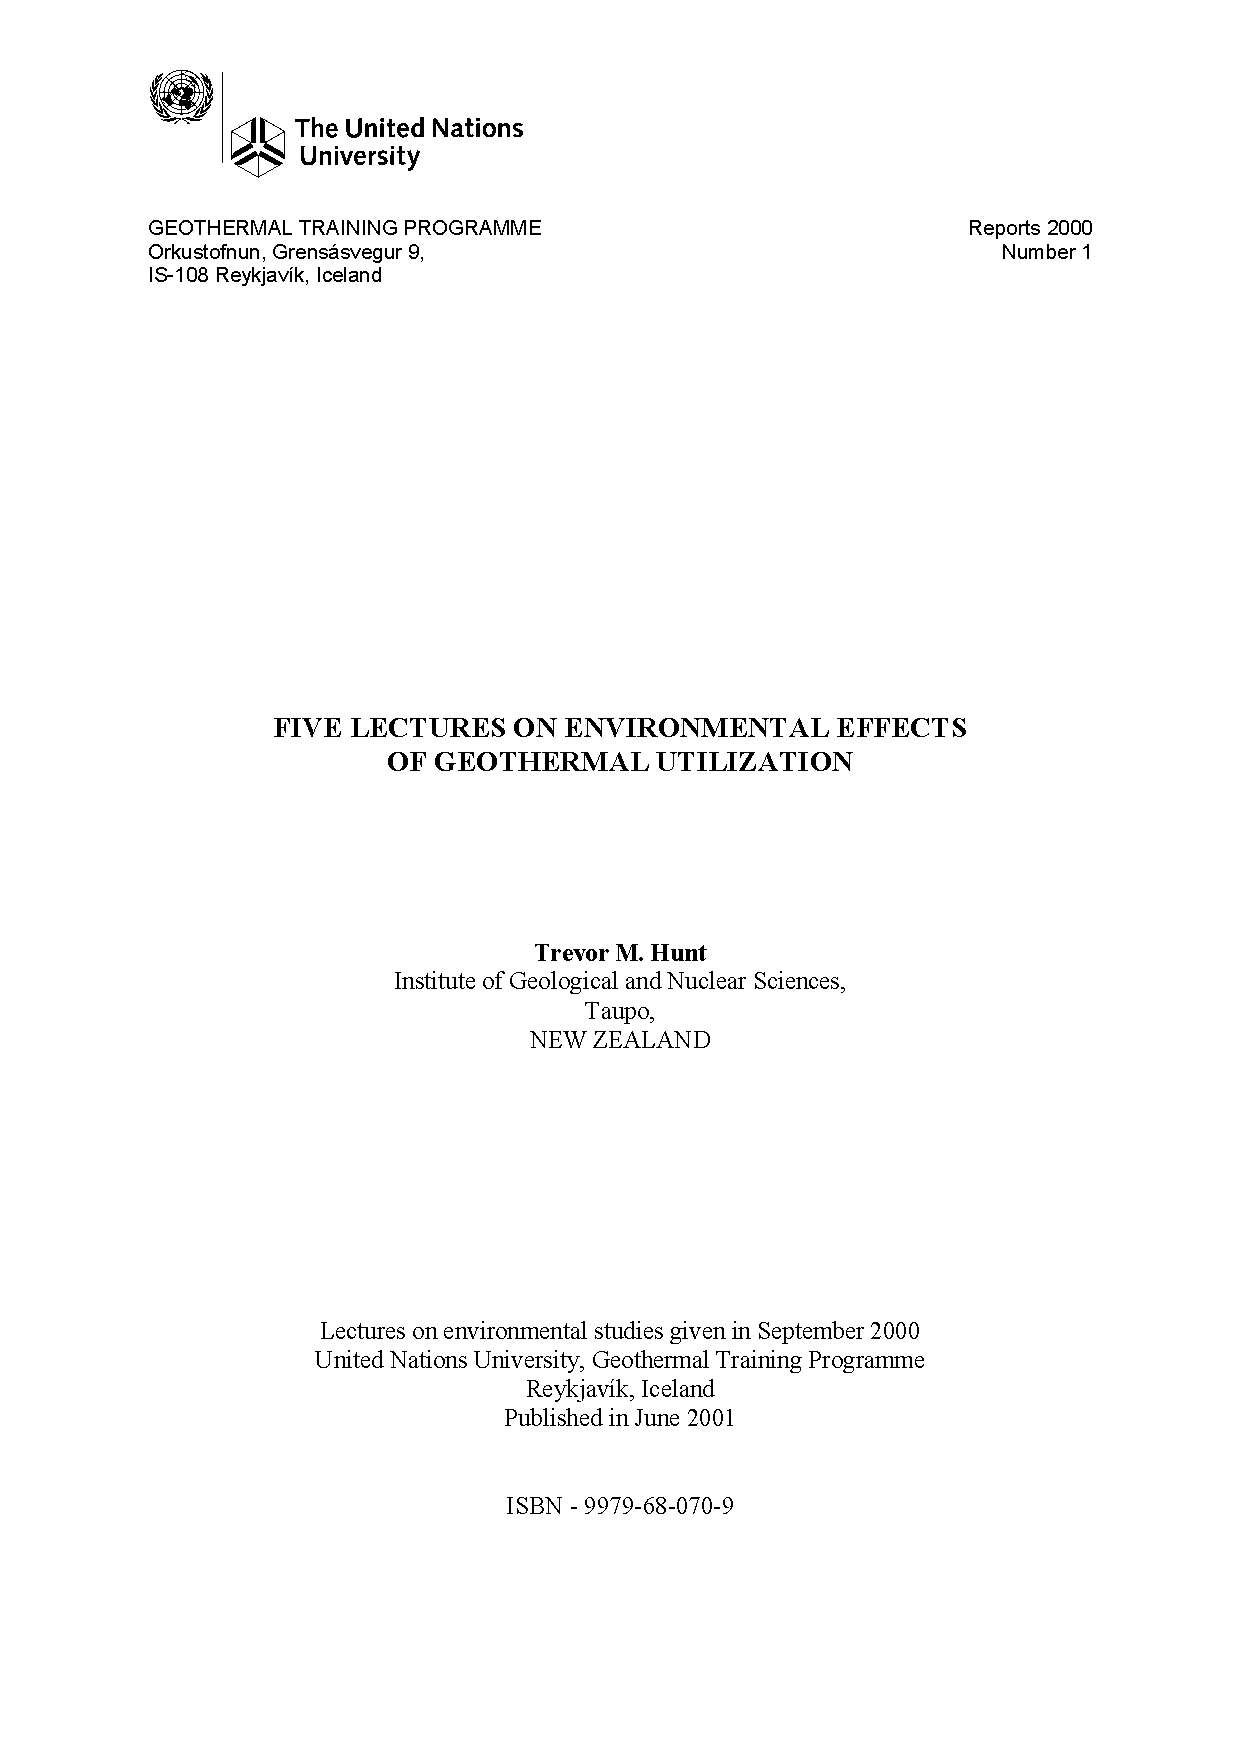
\includepdf[pages=-,fitpaper, angle=0]{./Tutorials/HuntSelect.pdf}
}

\end{document}
